\section{Demonstration scenario}
\label{sec:demonstr-scen}

This section contains a detailed walk through of a demonstration of using the verifier to verify a patch to AMP Challenge 10.

From the repository root directory, run the verifier in its docker container:
\begin{verbatim}
  docker run --rm -it -v `pwd`/demos/may-2023/challenge10:/challenge10 pate \
             --original /challenge10/challenge10.original.exe \
             --patched /challenge10/challenge10.patched.exe \
             -b /challenge10/challenge10.toml \
             --original-bsi-hints /challenge10/challenge10.json \
             --patched-bsi-hints /challenge10/challenge10.json \
             --original-csv-function-hints /challenge10/challenge10.csv \
             --patched-csv-function-hints /challenge10/challenge10.csv \
             -s transport\_handler
\end{verbatim}

The file \texttt{challenge10.toml} specifies additional metadata needed for verification.
Specifically it instructs the verifier to start decoding the binary in thumb mode.

The file \texttt{challenge10.json} contains symbol information extracted using the BSI tool.
This information is used to identify functions that should use stub semantics rather than be analyzed (e.g. libc calls).

The file \texttt{challenge10.csv} contains manually-defined symbol information that was not automatically extracted from the BSI tool.
This is necessary to handle some PLT stubs that were not identified.

The last line tells the verifier to start the analysis at the function corresponding to the symbol \texttt{transport\_handler}, which is known from the BSI symbol data.
This is the function in which the patch appears.

Once the verifier starts printing output it can be interrupted at any time by pressing ENTER, but will continue processing in the background.
Its results can then be interactively inspected as they become available.

See Section~\ref{sec:repl}for more information on how to interact with the verifier's Read-Eval-Print loop.

\noindent\textbf{Step 1: Select the entry point and wait}

 Select \texttt{1} to start the analysis from the \texttt{transport\_handler} function.
\begin{verbatim}
  Choose Entry Point
  0: Function Entry segment1+0x3ba9
  1: Function Entry "transport\_handler" (segment1+0x400c)
  ?> 1
  ....................
  0: Function Entry "transport\_handler" (segment1+0x400c) (User Request) (!).
  ...
\end{verbatim}

 The verifier then proceeds to print out each analysis step until user input is required.

 \noindent\textbf{Step 2: Choose a synchronization point}

 \begin{figure}[ht]
  \centerline{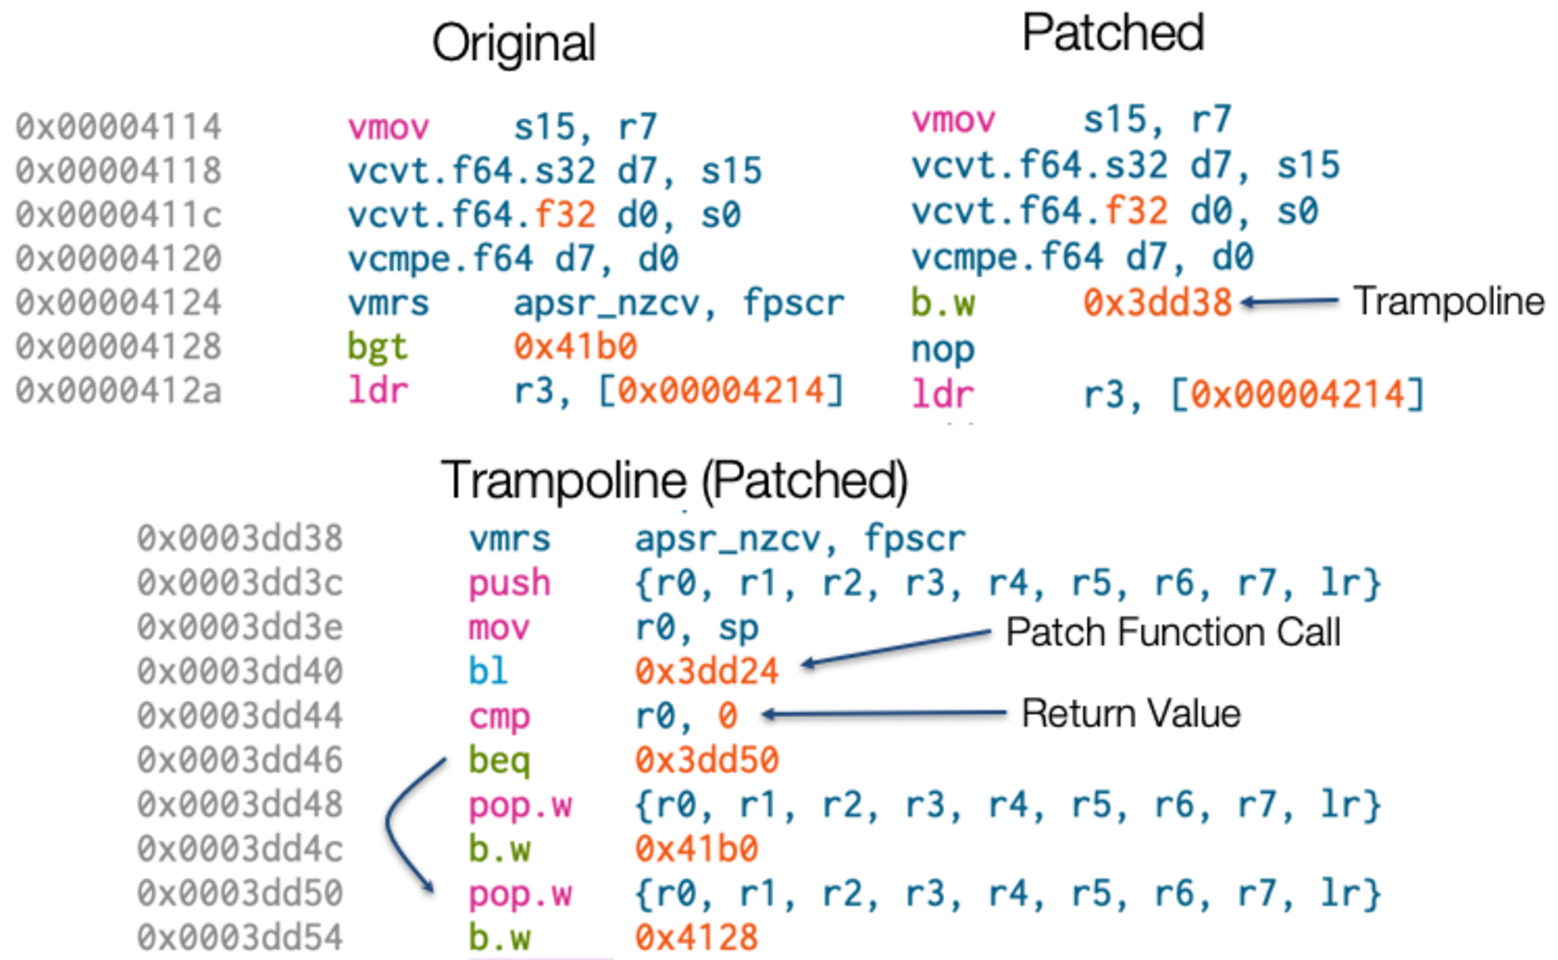
\includegraphics[width=0.9\linewidth]{patch.pdf}}
  \caption{Comparison of aligned regions in original and patched
    binaries for Challenge 10}
\label{fig:aligned}
\end{figure}

During the analysis of the block starting at \texttt{0x4114} the analysis encounters a control flow divergence.
This is an expected result of the patch, which, as shown in Figure~\ref{fig:aligned}, has inserted a trampoline starting at \texttt{0x4128}.
If the verifier is polling for output this will appear automatically, otherwise if the output was interrupted we can navigate to prompt by executing \texttt{top} followed by \texttt{goto\_prompt}:
\begin{verbatim}
  ?>goto\_prompt
  Control flow desynchronization found at: GraphNode segment1+0x4114
                   [ via: "transport\_handler" (segment1+0x400c) ]
  0: Ignore divergence (admit a non-total result)
  1: Assert divergence is infeasible
  2: Assume divergence is infeasible
  3: Remove divergence in equivalence condition
  4: Choose synchronization points
  5: Defer decision
  ?>
\end{verbatim}
Again, referring to Figure~\ref{fig:aligned} we can see where this happens in the code.
We can check the context of this choice by executing \texttt{up} then \texttt{up} to see the node that was being processed when this prompt was created.::
\begin{verbatim}
  ?>up
  ...
  ?>up
  segment1+0x4114 [ via: "transport\_handler" (segment1+0x400c) ] (Widening Equivalence Domains)
  0: Widening Equivalence Domains
  1: Modify Proof Node
  2: Predomain
  3: Observably Equivalent
  4: Block Exits (?)
  5:   Call to: "puts" (segment1+0x33ac) Returns to: "transport\_handler"
       (segment1+0x41b8) (original) vs. Call to: segment1+0x3dd24
      Returns to: "transport\_handler" (segment1+0x3dd44) (patched) (?)
  ?>
\end{verbatim}

Here we see that, from \texttt{0x4114} there are disagreeing block exits.
Specifically in the original program the block can exit with a call to \texttt{puts} while the patched function exits with a call to the anonymous function at \texttt{0x3dd24} (the inserted patch function).

To handle this, we need to instruct the verifier to perform a single-sided analysis on each program, and specify the point at which control flow re-synchronizes.
Specifically, we need to provide instruction addresses for the original and patched programs where, if execution reaches these addresses, both programs will resume in lockstep (i.e. all possible block exits (function calls) will be equal).
We navigate to the prompt with \texttt{goto\_prompt} and select \texttt{4: Choose synchronization points}.

We are then prompted to provide a pair of program points by selecting from a list of instructions.
With a separate analysis we can determine that the required synchronization points are \texttt{segment1+0x3dd44 (patched)} and \texttt{segment1+0x4128 (original)}.
As shown in Figure~\ref{fig:aligned}  at address \texttt{0x3dd44} (in the inserted trampoline), the patched program mirrors the branch instruction at \texttt{0x4128} in the original program.

Select these instructions from the list (one at a time) and the analysis will then continue.

\noindent\textbf{Step 3: Generate an equivalence condition}

The top-level nodes produced after this point are suffixed by \texttt{(original)} or \texttt{(patched)}, indicating which single-step analysis they correspond to.
After some analysis, the verifier prompts with another control flow desynchronization.
\begin{verbatim}
  Control flow desynchronization found at: GraphNode segment1+0x4128 (original) vs.
       segment1+0x3dd44 (patched) [ via: "transport\_handler" (segment1+0x400c) ]
  0: Ignore divergence (admit a non-total result)
  1: Assert divergence is infeasible
  2: Assume divergence is infeasible
  3: Remove divergence in equivalence condition
  4: Choose synchronization points
  5: Defer decision
  ?>
\end{verbatim}
This desynchronization indicates that control flow may still diverge between the original and patched programs after the synchronization point we provided.
This is exactly the intended result of our patch: after this point the program control flows \emph{may} be equal (i.e., in the case where the patch has simply recovered the original behavior of the program), but they may also be unequal (i.e., in the case where the patch has modified the program behavior).

Since this desynchronization precisely describes the non-equal branching behavior, we can exclude it from our analysis by asserting its negation as our generated *equivalence condition*.
This is option \texttt{3: Remove divergence in equivalence condition.}

After some analysis a similar prompt is given (corresponding to the inverse branching behavior), which we similarly handle by selecting \texttt{3} to assert the negation of this path condition.

The analysis then proceeds with this desynchronization omitted (and with a generated equivalence condition asserted at the synchronization point).

***********************************************************************

THIS IS THE POINT AT WHICH THE CURRENT DOCKER IMAGE (as of 7/27/23) throws an error.
So below here is not verified against actual execution.

***********************************************************************

\noindent\textbf{Step 4: Strengthening the equivalence domain}

After some time, the analysis eventually halts with a prompt indicating that a control flow difference has been found at \texttt{0x4181}.
With some investigation we can determine that this difference is spurious.
At the prompt, navigate to the toplevel node for \texttt{0x4181} via \texttt{up} then \texttt{up}, and select the option \texttt{2: Predomain}
\begin{verbatim}
  ?>up
  ..
  ?>up
  segment1+0x4181 [ via: "transport\_handler" (segment1+0x400c) ]
            (Widening Equivalence Domains)
  0: Widening Equivalence Domains
  1: Modify Proof Node
  2: Predomain
  3: Observably Equivalent
  4: Block Exits (?)
  5:   Call to: "err" (segment1+0x33ec) Returns to: "transport\_handler"
      (segment1+0x4191)
  6:   Call to: "err" (segment1+0x33ec) Returns to: "transport\_handler"
         (segment1+0x4191) (original) vs. Branch to: "transport\_handler"
         (segment1+0x402d) (patched) (?)
  ?>2
\end{verbatim}

The output here indicates that, although control flow is synchronized between the programs, several registers as well as global memory values are excluded from the equivalence domain (i.e., not known to be necessarily equivalence at this point).

The source of this inequivalence can be traced to the instruction immediately following the synchronization point at \texttt{0x412a} (\texttt{top} then \texttt{25} then \texttt{2}).
At this point, the equivalence domain has excluded \texttt{r0-r7} as well as the stack pointer and several stack slots.
This spurious inequivalence is a result of the trampoline saving and then restoring these registers onto the stack before resuming normal control flow.
The analysis has not retained enough context about the trampoline execution to automatically prove that this save/restore operation is sound.

We can instruct the verifier to strengthen the equivalence domain by explictly asserting that, at this program point, these registers are necessarily equivalent between the original and patched programs.
At the node for \texttt{0x412a} (\texttt{top} then \texttt{25}), select the option \texttt{1: Modify Proof Node}.
From this list we add an assertion by selecting \texttt{1: Assert condition}.

After providing this input, we are presented with the same control flow desynchronization prompt, which we now defer by selecting \texttt{4: Defer decision}, which will then present the prompt for the assertion we wish to add
\begin{verbatim}
  Include Register:
  0: r0
  1: r1
  2: r13
  3: r2
  4: r3
  5: r4
  6: r5
  7: r7
  8: Include Remaining Registers
  9: Exclude Remaining Registers
  ?> 8
\end{verbatim}

This is the list of registers that were excluded from the equivalence domain from \texttt{0x412a} Select \texttt{8} to include all of the given registers.
This choice results in an assertion that all of the user registers are necessarily equal between the original and patched programs when they both reach \texttt{0x412a}.
The analysis then proceeds by propagating the assertion up several nodes (indicated by the \texttt{Propagating Conditions} status), which is then eventually discharged.
The subsequent proof nodes are then re-checked under this new assertion, and correspondingly strengthened equivalence domain.

\noindent\textbf{Step 5: Propagating and interpreting the equivalence condition}

The verifier can now complete the analysis, prioviding a proof that the programs are exactly equivalent under the generated equivalence condition.
By default the condition is only asserted at exactly the location it is needed, however it can also be propagated to the entry point, in order to compute a sufficient condition at the beginning of the function call.

To do this, we navigate to the synchronization node (\texttt{top} then \texttt{57}) where we can see that an equivalence condition has been assumed.
However this is only in terms of the condition registers at this point.
Select \texttt{1: Modify Proof Node} and then \texttt{21:   Propagate fully}.

Then select \texttt{2: Handle pending refinements} at the next prompt to handle the requested action.
Once finished, the resulting equivalence condition can be examined by navigating to the node corresponding to the function entry point for \texttt{transport\_handler}.

%%% Local Variables:
%%% mode: latex
%%% TeX-master: "user-manual"
%%% End:
